To reduce bias and variance in our model we use best subset selection, as we discussed in section \ref{sec_level1}. Looking at the results in table \ref{tab:BestSubset} we observe that the predictor $Rcyl$ gets added first, followed by $mgfe$/$ch$, $vphi$ and $age$. We already predicted that $Rcyl$ and $vphi$ were important predictors, and it makes sense that the model chooses almost randomly between the concentration predictors, since they are highly correlated.
\begin{table}[h!]
\caption{Best subset selection results for k predictors}
\label{tab:BestSubset}
\resizebox{\columnwidth}{!}{
\begin{tabular}{lrrrrrrrrrrrrrrr}
\toprule
 & Rcyl & age & cfe & ch & feh & intercept & mass & mgh & ofe & oh & phi & vRcyl & vphi & vz & z \\
\midrule
0 & - & - & - & - & - & -1.53 & - & - & - & - & - & - & - & - & - \\
1 & 0.48 & - & - & - & - & -3.09 & - & - & - & - & - & - & - & - & - \\
2 & 0.50 & - & -5.19 & - & - & -1.55 & - & - & - & - & - & - & - & - & - \\
3 & 0.48 & - & - & -1.20 & - & -3.57 & - & - & - & - & - & - & 0.00 & - & - \\
4 & 0.46 & - & -8.17 & - & - & -6.12 & - & - & 10.88 & - & - & - & 0.00 & - & - \\
5 & 0.40 & -0.34 & - & -13.69 & - & -0.88 & - & 12.86 & - & - & - & - & 0.00 & - & - \\
6 & 0.39 & -0.43 & - & -12.21 & - & 1.42 & - & 20.08 & - & -9.16 & - & - & 0.00 & - & - \\
7 & 0.39 & -0.44 & 7.09 & -16.67 & - & -0.47 & - & 24.66 & - & -9.32 & - & - & 0.00 & - & - \\
8 & 0.39 & -0.44 & 7.13 & -16.68 & - & -0.47 & - & 24.69 & - & -9.34 & - & - & 0.00 & - & 0.10 \\
9 & 0.39 & -0.44 & 7.19 & -16.67 & - & -0.48 & - & 24.72 & - & -9.39 & - & - & 0.00 & -0.00 & 0.09 \\
10 & 0.39 & -0.44 & - & -9.46 & 78.85 & -0.55 & - & 24.67 & 86.16 & -95.40 & - & - & 0.00 & -0.00 & 0.09 \\
11 & 0.39 & -0.44 & - & -9.49 & 80.23 & -0.48 & -0.00 & 24.34 & 87.48 & -96.41 & - & - & 0.00 & -0.00 & 0.09 \\
12 & 0.39 & -0.44 & -48.14 & 38.64 & 48.79 & -0.47 & -0.00 & 24.32 & 104.13 & -113.08 & - & - & 0.00 & -0.00 & 0.09 \\
13 & 0.39 & -0.44 & -49.49 & 40.04 & 47.26 & -0.70 & -0.00 & 24.17 & 103.99 & -112.78 & 0.00 & - & 0.00 & -0.00 & 0.08 \\
14 & 0.39 & -0.44 & -49.81 & 40.31 & 46.39 & -0.70 & -0.00 & 24.16 & 103.41 & -112.16 & 0.00 & -0.00 & 0.00 & -0.00 & 0.08 \\
\bottomrule
\end{tabular}
}
\end{table}


If we take a look at figure \ref{fig:BicAicAccuracy}
% \begin{figure}
%     \centering
%     \includegraphics[width=0.5\linewidth]{}
%     \caption{Caption}
%     \label{fig:enter-label}
% \end{figure}
we observe that the accuracy is highest for 10 predictors, but stays pretty much the same after adding $Rcyl$, where BIC is  at a minimum at 6 predictors and AIC keeps falling, but very little. This leads to the conclusion that the best number of predictors is 6. The accuracies are actually pretty low if you compare with the most naive classifier, which only predicts non-migrators, with an accuracy of 82,4\%, since the dataset is skewed towards non-migrators.

\begin{figure}[h!]
    \centering
    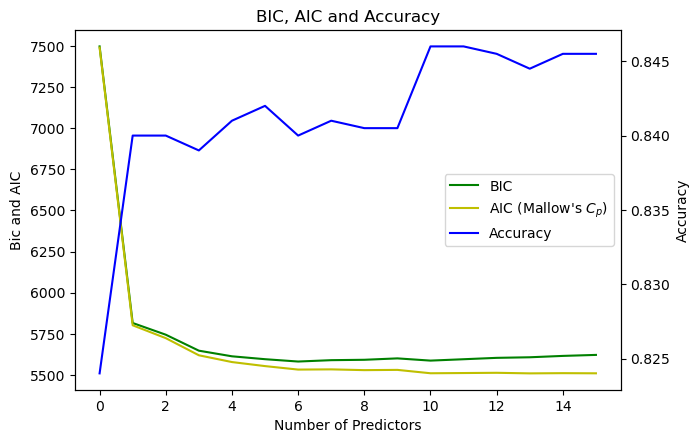
\includegraphics[width=0.8\columnwidth]{Plots/BIC, AIC, ACC all 15.png}
    \caption{BIC, AIC and Accuracy as a function of number of predictors in best subset selection}
    \label{fig:BicAicAccuracy}
\end{figure}

% We then perform logistic regression on the full dataset, both using all of the predictors and yielding an accuracy of 83.1\% and only using the predictors found in best subset selection yielding an accuracy of 82,3\%, which curiously is lower than that of the most naive classifier that only predicts non-migrators, with an accuracy of 82,4\%. Both are actually lower than what we see from the models trained on sampled data, although this performance drop is likely due to not removing outliers from the full dataset and generally we can conclude that logistic regression is not a good fit for predicting migrators.